\documentclass{article}
\usepackage{amsmath}
\usepackage{fullpage}
\usepackage{makecell}
\usepackage{multirow}
\usepackage{tikz}

\title{Title}
\author{Author's Name}
\date{\today}

\newcounter{question}
\newcommand{\question}{\stepcounter{question}\section*{Question \thequestion}}

\newcounter{subquestion}[question]
\newcommand{\subquestion}{\stepcounter{subquestion}\subsection*{Part \thesubquestion}}

\newcounter{subsubquestion}[subquestion]
\renewcommand{\thesubsubquestion}{\alph{subsubquestion}}
\newcommand{\subsubquestion}{\stepcounter{subsubquestion}\subsubsection*{(\thesubsubquestion)}}

\usetikzlibrary {automata,positioning}

\begin{document}

\maketitle

\question
\subsubquestion
hello
\subsubquestion
\begin{verbatim}
hello
\end{verbatim}
\subsubquestion
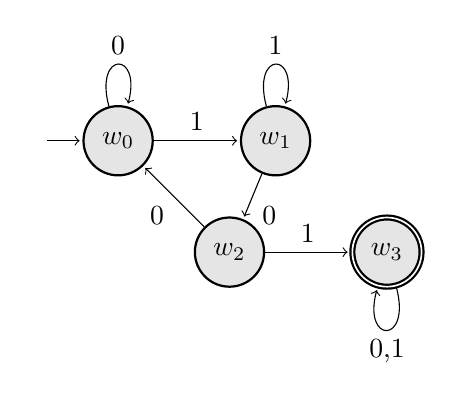
\begin{tikzpicture}[shorten >=1pt,node distance=2cm,on grid,auto,initial text=,
                    every state/.style={thick,fill=gray!20}]
  \node[state,initial]   (q_0)                      {$w_0$};
  \node[state]           (q_1) [right=of q_0]       {$w_1$};
  \node[state]           (q_2) [below right=of q_0] {$w_2$};
  \node[state,accepting] (q_3) [right=of q_2]       {$w_3$};

  \path[->] (q_0) edge [loop above] node {0}   ()
                  edge              node {1}   (q_1)
            (q_1) edge              node {0}   (q_2)
                  edge [loop above] node {1}   (q_1)
            (q_2) edge              node {0}   (q_0)
                  edge              node {1}   (q_3)
            (q_3) edge [loop below] node {0,1} (q_3);
\end{tikzpicture}
\subsubquestion
\scalebox{0.9}{
\begin{tabular}{|c|c|c|c|}
\hline
\multicolumn{2}{|c|}{Hello} & \multicolumn{2}{|c|}{$\epsilon$} \\
\hline
hello & $w_1$ & hello & $w_1$ \\
\hline
\end{tabular}
}

\question
\subquestion
\begin{align*}
\langle\text{hello}\rangle&\models\texttt{START }\langle\text{middle}\rangle\texttt{ END}\mid\epsilon\\
\langle\text{middle}\rangle&\models\texttt{B}\mid\texttt{A}
\end{align*}
\subquestion
\begin{tabular}{|c|c|}
\hline
\textbf{hello} & \textbf{hello} \\
\hline\hline
\makecell{$\langle\text{hello}\rangle\models$\\\texttt{START }\\$\langle\text{middle}\rangle$\\\texttt{ END}} & hello \\
\makecell{$\langle\text{hello}\rangle\models$\\$\mid\epsilon$} & hello \\
\hline
\end{tabular}

\end{document}
